\documentclass[a4paper,onecolumn]{extarticle}
\usepackage{geometry}
\usepackage[page,toc,titletoc,title]{appendix}
\usepackage{url}
\usepackage{caption}
\usepackage{subfigure}
\usepackage{subcaption}
\usepackage[sc]{mathpazo} % Use the Palatino font
\usepackage[T1]{fontenc} % Use 8-bit encoding that has 256 glyphs
\usepackage[utf8]{inputenc} % Use utf-8 as encoding
\linespread{1.05} % Line spacing - Palatino needs more space between lines
\usepackage{microtype} % Slightly tweak font spacing for aesthetics
\usepackage[spanish, activeacute]{babel}
 \decimalpoint
% \usepackage[hmarginratio=1:1,top=32mm,columnsep=20pt]{geometry} % Document marginshttps://www.overleaf.com/project/60211b96f72a79d4c7515e93
% \usepackage[hang, small,labelfont=bf,up,textfont=it,up]{caption} % Custom captions under/above floats in tables or figures
\usepackage{verbatim} % comentarios
\usepackage{listings}
\usepackage{xcolor}
\usepackage{wrapfig}
\lstset{
    inputencoding=utf8,
    frame=single,
    basicstyle=\fontsize{7}{10}\selectfont\ttfamily,
    basicstyle=\ttfamily\small,
    keywordstyle=\color{blue}\bfseries,
    identifierstyle=\color{black},
    commentstyle=\color{gray}\itshape,
    stringstyle=\color{red},
    numbers=left,
    numberstyle=\tiny\color{gray},
    stepnumber=1,
    numbersep=10pt,
    showspaces=false,
    showstringspaces=false,
    breaklines=true,
    breakindent=0pt,
    breakatwhitespace=false,
    tabsize=2,
    captionpos=b,
    literate={á}{{\'a}}1
        {ã}{{\~a}}1
        {é}{{\'e}}1
        {ó}{{\'o}}1
        {í}{{\'i}}1
        {ñ}{{\~n}}1
        {¡}{{!`}}1
        {¿}{{?`}}1
        {ú}{{\'u}}1
        {Í}{{\'I}}1
        {Ó}{{\'O}}1
}
\setlength{\parskip}{0.8em}
\usepackage{natbib}
\usepackage{enumitem}
% \setlist[itemize]{noitemsep} % Make itemize lists more compact
% \usepackage{abstract} % Allows abstract customization
% \renewcommand{\abstractnamefont}{\normalfont\bfseries} % Set the "Abstract" text to bold
% \renewcommand{\abstracttextfont}{\normalfont\small\itshape} % Set the abstract itself to small italic text
\usepackage{titlesec}

\usepackage{fancyhdr} % Headers and footers
\pagestyle{fancy} % All pages have headers and footers
\fancyhead{}
\lhead{Hugo Gómez Sabucedo}
\rhead{Minería de datos y modelización predictiva}

\renewcommand{\footrulewidth}{0.2pt}
\usepackage{titling} % Customizing the title section
\usepackage[breaklinks=true]{hyperref} % For hyperlinks in the PDF
%\usepackage{array}
%\newcolumntype{C}[1]{>{\centering\let\newline\\\arraybackslash\hspace{0pt}}m{#1}}
\usepackage{graphicx}
%\usepackage{lipsum} % NO NECESARIO LUEGO
%\usepackage{amsmath}
%\usepackage{wrapfig}
%\usepackage{multicol}
%\usepackage{bm}


\let\stdsection\section
\renewcommand\section{\newpage\stdsection}

%-------------------------------------------------------------------------------
%	TITLE SECTION
%-------------------------------------------------------------------------------

\setlength{\droptitle}{-4\baselineskip} % Move the title up



\title{\begin{center} \Huge Minería de datos y modelización predictiva \end{center}} % Article title
\author{
    \textsc{\Huge Hugo Gómez Sabucedo} \\ % Your name
    \large \href{mailto:hugogomezsabucedo@gmail.com}{hugogomezsabucedo@gmail.com} \\ [2ex] % Your email address
    \Large \textbf{Máster Big Data, Data Science \& Inteligencia Artificial} \\
    \normalsize Curso 2024-2025 \\
    \large Universidad Complutense de Madrid
}
\date{} % Leave empty to omit a date

\begin{document}
% Print the title
\maketitle
%\newpage
\tableofcontents
%\newpage
\begin{sloppypar}

%-------------------------------------------------------------------------
%	DOCUMENT
%-------------------------------------------------------------------------

\section{Introducción y análisis} \label{introduccion}
\subsection{Introducción} \label{intro}
En este ejercicio analizaremos el conjunto de datos de \texttt{penguins} disponible en la librería \texttt{seaborn} de Python. Este conjunto de datos contiene
observaciones de diferentes ejemplares de pingüinos, para cada uno de los cuales se recoge su especie (`Adelie`, `Chinstrap` o `Gentoo`) la isla en la que se 
encuentra (`Biscoe`, `Dream` y `Torgensen`), la longitud de su pico (\textit{bill\_length\_mm}, en milímetros), la profundidad de su pico 
(\textit{bill\_depth\_mm}, también en milímetros), la longitud de su aleta (\textit{flipper\_length\_mm}, en milímetros), su masa corporal 
(\textit{body\_mass\_g}, en gramos), y su género (que puede ser `Male` para macho, `Female` para hembra, o `NaN` si no está disponible). El objetivo de este 
ejercicio es aplicar las diferentes técnicas de reducción de dimensionalidad y de agrupamiento, para ver si se pueden definir grupos de pingüinos con 
características similares.

En primer lugar, observamos una pequeña muestra de los datos para comprobar su estructura. Haciendo un \texttt{.head(5)} vemos los 5 primeros registros, en 
donde se observan algunos detalles interesantes. Observamos que hay valores perdidos (NaN) no sólo en el género, sino que hay un pingüino que tiene todos 
los valores perdidos, para el que no tenemos ningún dato. Tendremos que analizar la mejor estrategia para tratar este caso.
\begin{table}[h!]
    \begin{tabular}{|c c c c c c c|}
        \hline
        \textbf{species} & \textbf{island} & \textbf{bill\_length\_mm} & \textbf{...} & \textbf{flipper\_length\_mm} & \textbf{body\_mass\_g} & \textbf{sex} \\
        \hline
        Adelie & Torgersen & 39.1 & ... & 181.0 & 3750.0 & Male \\
        Adelie & Torgersen & 39.5 & ... & 186.0 & 3800.0 & Female \\
        Adelie & Torgersen & 40.3 & ... & 195.0 & 3250.0 & Female \\
        Adelie & Torgersen & NaN & ... & NaN & NaN & NaN \\
        Adelie & Torgersen & 36.7 & ... & 193.0 & 3450.0 & Female \\
        \hline
    \end{tabular}
    \caption{}
    \label{tab:headDF}
\end{table}

En la figura \ref{fig:descriptivos} se puede observar un análisis descriptivo de las variables numéricas. Lo primero a destacar es que se observan 2 NaN en 
cada variable, lo cual nos podría indicar que tenemos, además del pingüino que vimos anteriormente, otro con todos los datos faltantes. Esto se refuerza 
viendo que el conteo de las variables es de 342, cuando en el conjunto de datos tenemos 344 pingüinos. Respecto a la distribución de los datos, vemos que las 
dos primeras variables son bastante simétricas, con coeficientes de asimetría próximos a 0. Para las otras dos variables, se observa una simetría positiva, 
un poco más pronunciada en el caso del peso, pero en general es una distribución también simétrica. Tampoco se observan valores atípicos en los datos.
\begin{center}
    \begin{figure}[h!]
        \centering
        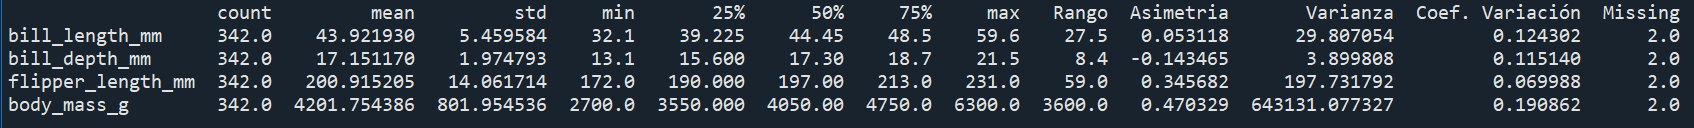
\includegraphics[width=\textwidth]{graficos/descriptivos.png}
        \caption{Análisis descriptivo de los datos}
        \label{fig:descriptivos}
    \end{figure}
\end{center}

Respecto al tratamiento de los valores NaN, se han decidido eliminar por completo aquellos registros con algún valor missing, ya que la cantidad que se ha 
observado de los mismos es realmente pequeña. Como se comentó, se detectan dos ejemplares con todos los datos missing, además de nueve de ellos para los que 
falta el sexo. Es una proporción escasa de los datos, por lo que su eliminación no supondría una gran pérdida de información. Aún así, se recalca que, para 
el tratamiento de los valores missing, se podría aplicar algún algoritmo que los imputase manteniendo la proporción de género que hay originalmente. Se observa 
una distribución prácticamente simétrica, con 165 pingüinos hembra y 168 machos, por lo que, de los 9 pingüinos que tienen el sexo missing, podríamos establecer 
para cinco de ellos el sexo `Female`, y el sexo `Male` para cuatro de ellos, y teniendo en cuenta la especie, manteniendo así el equilibrio.

Por último, convertiremos los valores de la variable sexo, ya que es dicotómica, mapeando el género macho como 1 y el género hembra como 0, de forma que 
podamos usar esta variable también en el análisis, proporcionándonos una nueva característica para los datos. De esta forma, sólo quedarían como variables 
categóricas la especie y la isla, las cuales se eliminarán también, ya que no tendría sentido mantenerlas. De todas formas, se guarda una copia del dataframe, 
ya que resultará útil de cara al análisis de los resultados ver en qué isla o de que especie es cada pingüino y cuál predomina en cada grupo.

\subsection{Correlaciones entre las variables}\label{correlaciones}
\begin{wrapfigure}[15]{l}{7cm}
    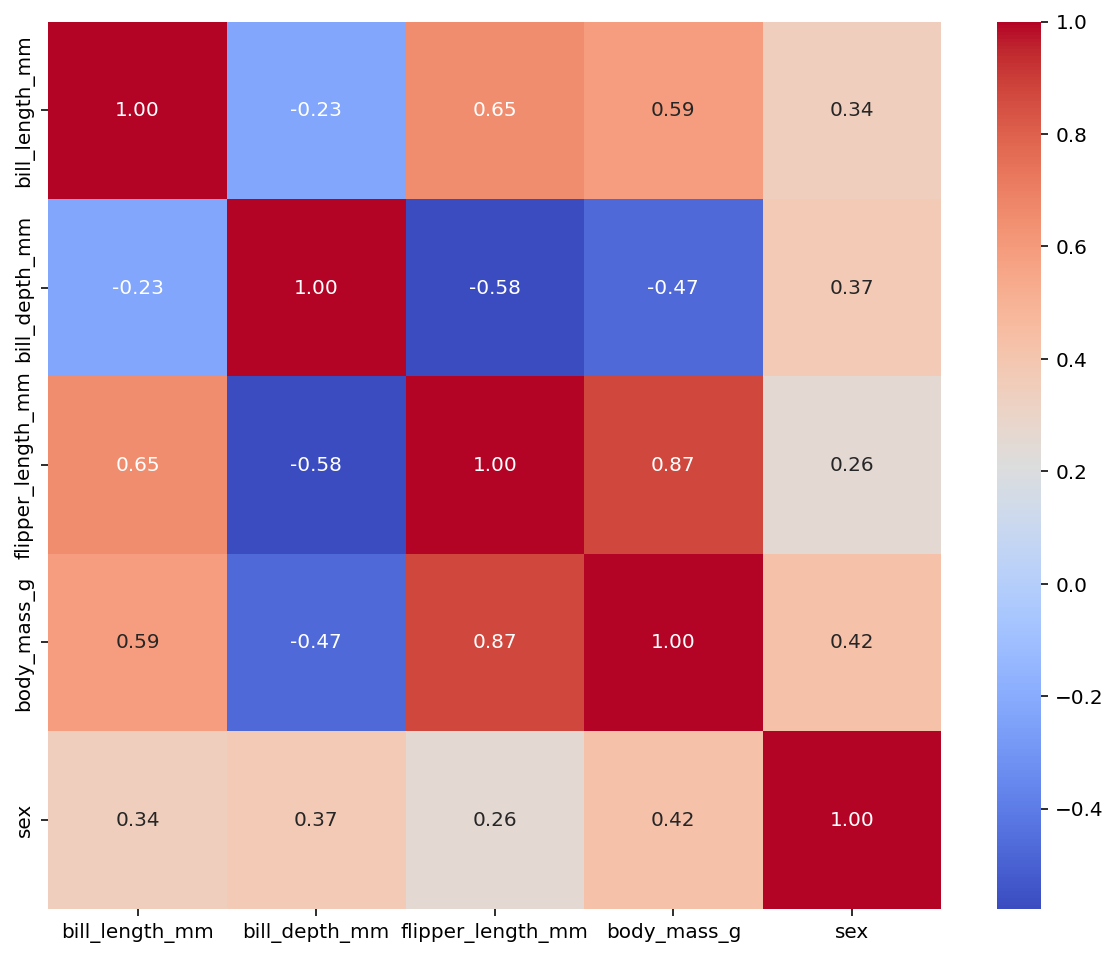
\includegraphics[width=7cm]{graficos/correlacion.png}
    \small{\caption{Matriz de correlacion}}
    \label{correlacion}
\end{wrapfigure} 
Si representamos la matriz de correlaciones, observamos una relación positiva fuerte entre el peso y la longitud de la aleta, así como entre la longitud del 
pico y el peso y la longitud de la aleta. Esto significa, por ejemplo, que los pingüinos que tienen mayor peso tienden a tener una aleta más larga. Sin embargo, 
entre el peso y la longitud de la aleta se observa una correlación negativa con la profundidad del pico, lo que nos indica que, cuanto más profundo es el pico, 
menos pesa y más corta tiene la aleta el pingüino. Cabe destacar también la relación negativa entre la longitud y la anchura del pico, lo cual indicaría que 
los pingüinos tienen picos anchos y cortos, o largos y estrechos.

\section{Análisis PCA} \label{analisisPCA}
\subsection{Análisis inicial} \label{PCAinicial}
Para comenzar con el análisis PCA o de componentes principales, lo primero que haremos será estandarizar los datos, ya que las escalas de las variables originales 
son distintas (unas unidades en mm, otras en gramos...), y uno de los requisitos para poder aplicar el PCA es que los datos estén en la misma escala o 
estandarizados. Como vimos en \ref{intro}, los datos no presentan valores atípicos, y también se han limpiado de valores perdidos, por lo que los datos cumplen 
todos los requisitos para aplicar el PCA.

Creamos el PCA con cuatro componentes, el número máximo que se indica, y calculamos los autovalores, la varianza explicada y la varianza acumulada, recogiéndose 
en la tabla \ref{tab:autovalores}.
\begin{table}[h!]
    \centering
    \begin{tabular}{|c|c|c|c|}
        \hline
        & \textbf{Autovalores} & \textbf{Varianza explicada} & \textbf{Varianza Acumulada} \\
        \hline
        Componente 1 & 2.844160 & 0.567124 & 0.567124 \\
        Componente 2 & 1.411420 & 0.281436 & 0.848560 \\
        Componente 3 & 0.486707 & 0.097049 & 0.945609 \\
        Componente 4 & 0.172850 & 0.034466 & 0.980075 \\
        \hline
    \end{tabular} 
    \caption{Tabla con autovalores}
    \label{tab:autovalores}
\end{table}

\begin{wrapfigure}[14]{l}{7.5cm}
    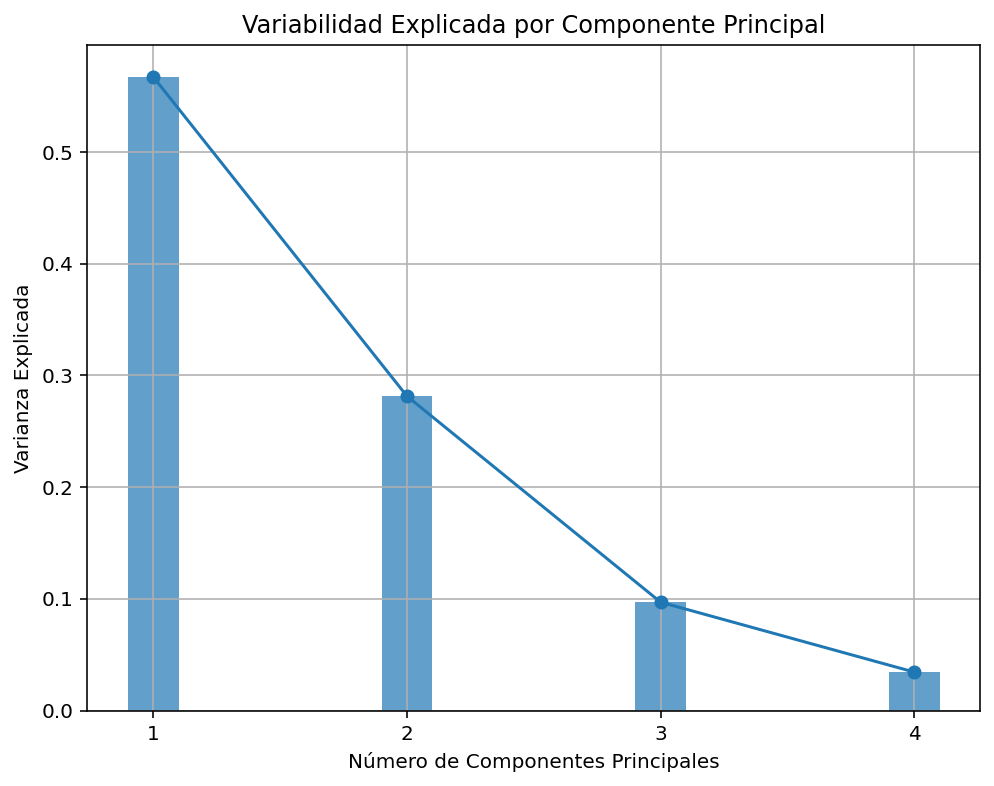
\includegraphics[width=7.5cm]{graficos/varExplicada.png}
    \small{\caption{Variabilidad Explicada} \label{fig:varExplicadaGraf}}
\end{wrapfigure} 
Respecto a los autovalores, nos indican la cantidad de varianza explicada por cada uno de los componentes, de forma que cuanto mayor sea implica que esa 
componente retiene una gran cantidad de información de los datos originales. Estos valores son más elevados para los dos primeros componentes, que, además,
si analizamos la varianza explicada (también en la figura \ref{fig:varExplicada}) y la acumulada, vemos que entre los dos explican casi el 85\% de la 
variabilidad de las variables originales. Para elegir el número adecuado de componentes, tenemos en cuenta los siguientes criterios:
\\
\\
\begin{itemize}
    \item Que los autovalores de las componentes sean mayores a 1. En este caso, sólo lo cumplen las componentes 1 y 2.
    \item Que los componentes expliquen al menos entre el 80\% y el 90\% de los datos originales (usando la varianza acumulada). Con las dos primeras
    componentes tenemos un 84.5\% de la varianza explicada.
    \item Observando el gráfico de la variabilidad explicada (figura \ref{fig:varExplicadaGraf}).
\end{itemize}

Por lo tanto, aplicando todos estos criterios, viendo que en la tercera componente del gráfico del codo ya no se aprecia una ganancia significativa de 
información (contribuye apenas en un 10\%) y que, además, su autovalor es menor que 1, se determina que el \textbf{número adecuado de componentes es 2}.

\subsection{PCA sobre los datos estandarizados} \label{PCAest}
Una vez que hemos determinado el número de componentes adecuados como 2, repetimos el PCA con este número de componentes principales. Obtenemos los autovectores
para cada componente, así como las correlaciones entre cada componente y las variables originales (para ver que variables tienen más peso en cada componente), 
y el cuadrado de esta correlación (para ver qué proporción de la varianza de esa variable es explicada por ese componente). Los resultados obtenidos se recogen 
en la tabla \ref{tab:tablaPCA}. Sus representaciones gráficas se encuentras englobadas en la figura \ref{fig:multiplesGraficas}.
\begin{table}[h!]
    \begin{tabular}{|c|c|c|c|c|c|c|}
        \hline
        \textbf{Variable} & \textbf{Autovector 1} & \textbf{Autovector 2} & \textbf{Corr. C1}  & \textbf{Corr. C2} & \textbf{$cos^2$ C1} & \textbf{$cos^2$ C2} \\
        \hline
        bill\_length\_mm\_z    & 0.462289  & 0.168869  & 0.778463  & 0.200320  & 0.606004 & 0.040128 \\
        bill\_depth\_mm\_z     & -0.331708 & 0.652723  & -0.558574 & 0.774291  & 0.312005 & 0.599527 \\
        flipper\_length\_mm\_z & 0.563897  & -0.094552 & 0.949563  & -0.112162 & 0.901669 & 0.012580 \\
        body\_mass\_g\_z       & 0.554251  & 0.047941  & 0.933320  & 0.056869  & 0.871085 & 0.003234 \\
        sex\_z                 & 0.226018  & 0.730888  & 0.380598  & 0.867013  & 0.144855 & 0.751712 \\
        \hline
    \end{tabular} 
    \caption{Métricas del PCA}
    \label{tab:tablaPCA}
\end{table}

En lo que respeta a la interpretación de los resultados, por un lado tenemos los autovectores, que indican la contribución de cada variable original a una 
componente en concreto. Esto lo vemos también en la figura \ref{fig:cargas}, donde vemos que las variables que más contribuyen en el autovector 1 son 
\textit{`flipper\_length\_mm\_z`}, \textit{`body\_mass\_g\_z`} y \textit{`bill\_length\_mm\_z`}, mientras que \textit{`sex\_z`} y
\textit{`bill\_depth\_mm\_z`} tienen una menor contribución. Lo contrario ocurre en el caso del autovector 2. Apoyándonos también en la figura 
\ref{fig:vectores}, esto nos sugiere que la primera componente está relacionada con el tamaño en general del pingüino (longitud de la aleta y masa, así como 
longitud de pico), mientras que la segunda componente captura más información sobre las diferencias entre los pingüinos machos y hembra. De esta forma, las 
especies de pingüinos más grandes tomarán también valores más grandes en la componente 1, mientras que en la componente 2 tomarán valores más altos aquellas 
especies con picos más profundos o que tengan diferencias más marcadas entre los machos y las hembras. También observamos la varianza explicada de cada 
variable (figura \ref{fig:varExplicada}) y el gráfico de dispersión de las observaciones en base a cada variable (figura \ref{fig:dispersionBasico}).

\begin{center}
    \begin{figure}[h!]
        \centering
        \begin{minipage}{0.45\textwidth}
            \centering
            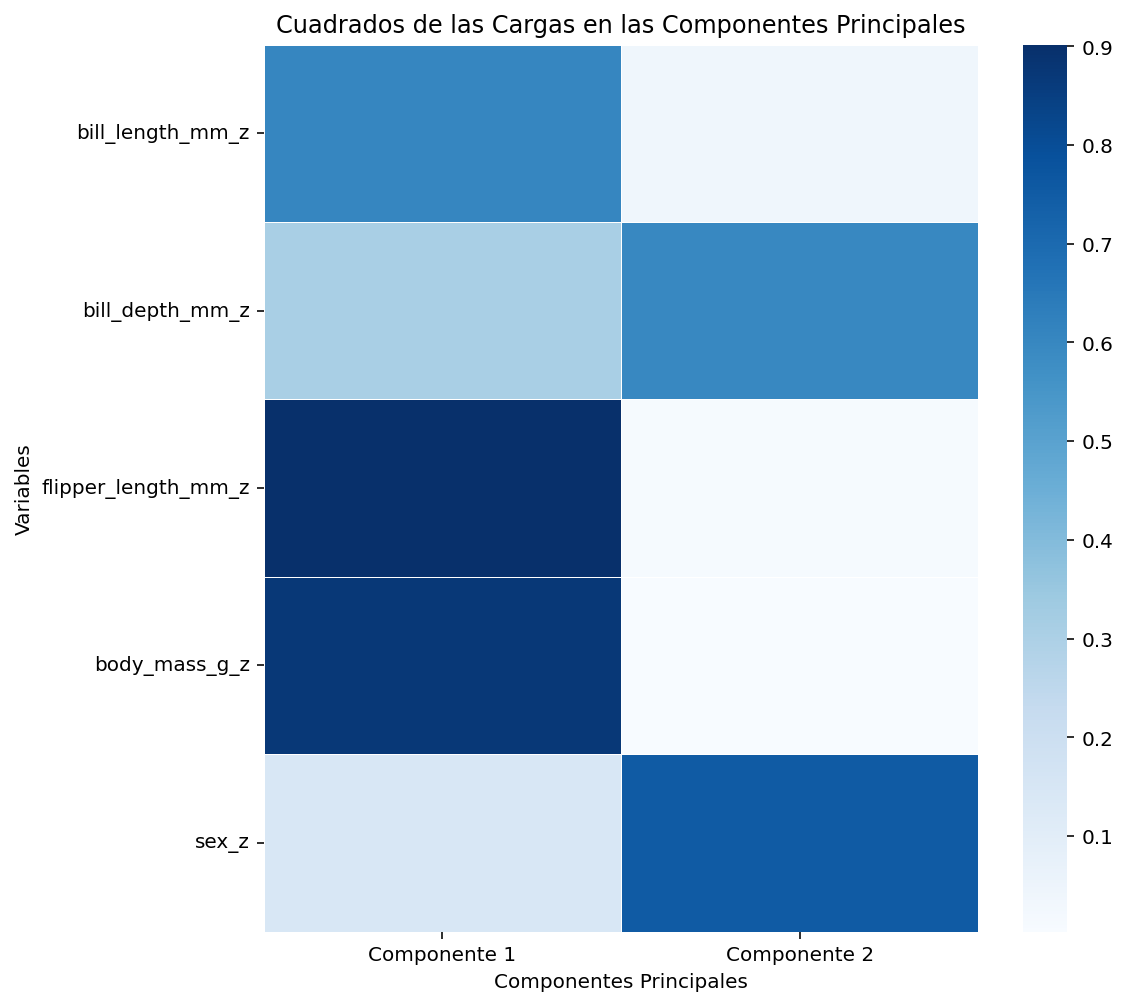
\includegraphics[width=\textwidth]{graficos/cargasComponentes.png}
            \caption{\small{Cargas en las componentes principales}}
            \label{fig:cargas}
        \end{minipage}
        \hspace{0.005\textwidth} % Espacio entre las imágenes
        \begin{minipage}{0.45\textwidth}
            \centering
            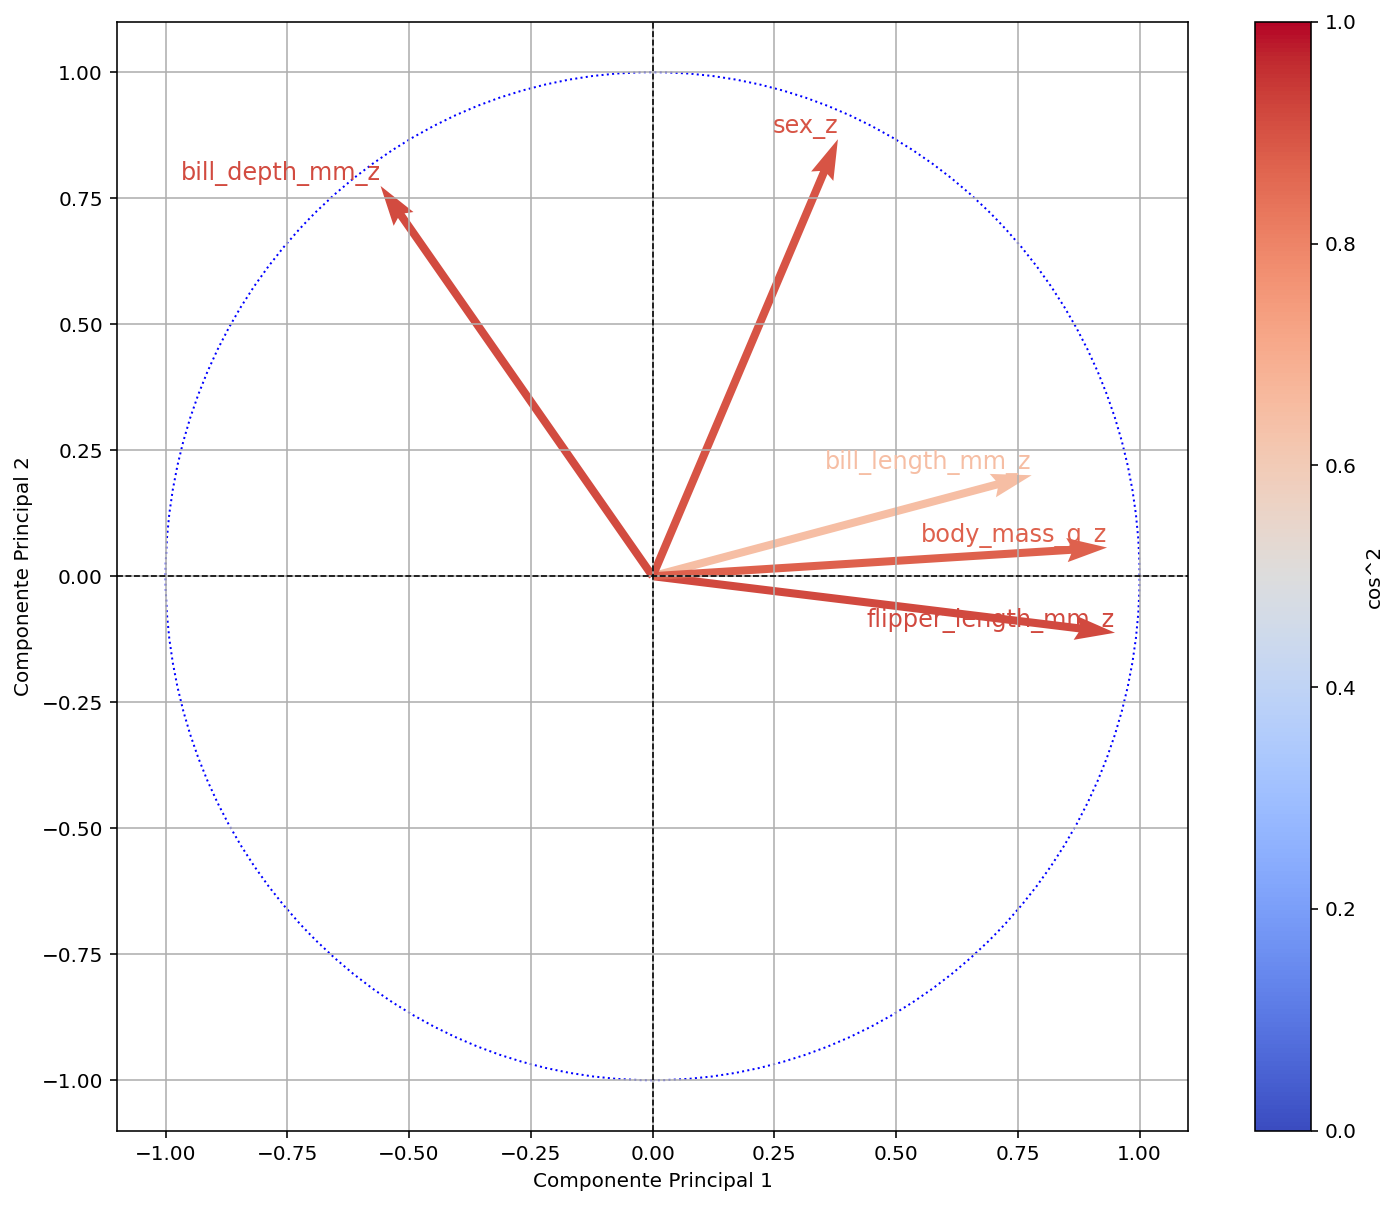
\includegraphics[width=\textwidth]{graficos/correlacionVectores.png}
            \caption{\small{Autovectores para componentes principales}}
            \label{fig:vectores}
        \end{minipage}
        \centering
        \begin{minipage}{0.45\textwidth}
            \centering
            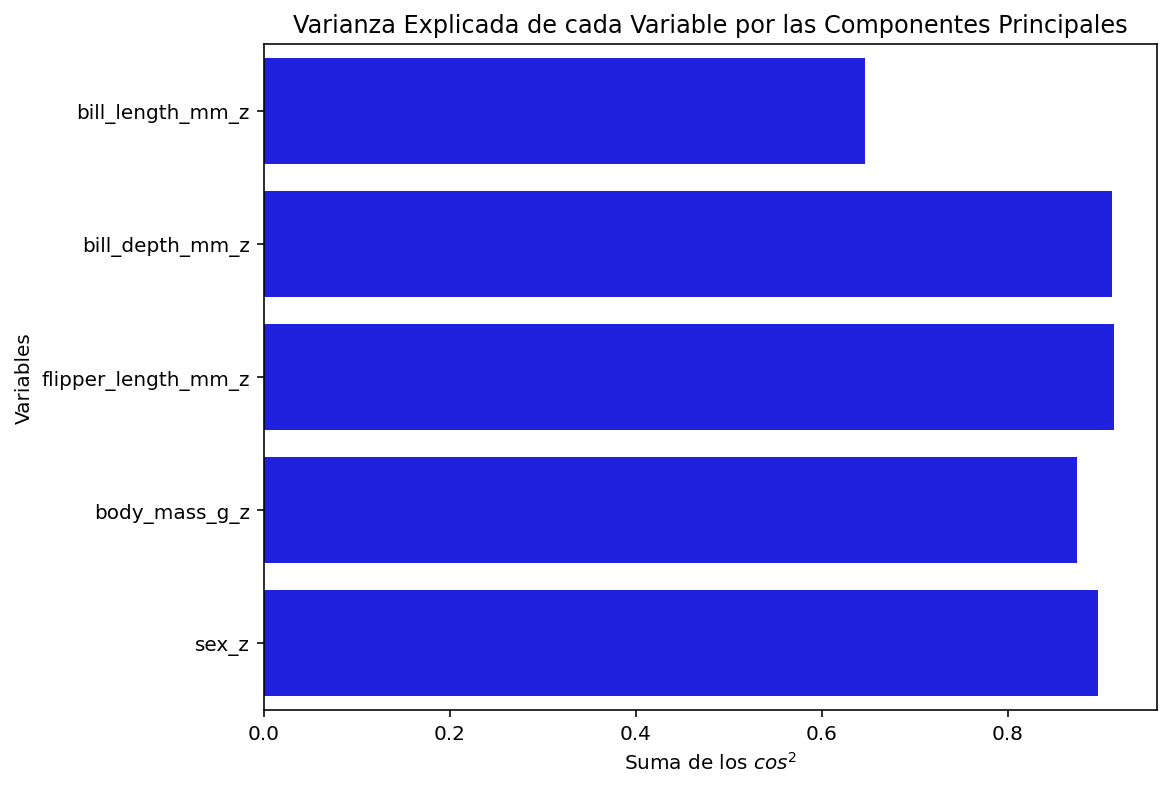
\includegraphics[width=\textwidth]{graficos/VarExplicadaCos.png}
            \caption{\small{Varianza explicada de cada variable}}
            \label{fig:varExplicada}
        \end{minipage}
        \hspace{0.005\textwidth} % Espacio entre las imágenes
        \begin{minipage}{0.45\textwidth}
            \centering
            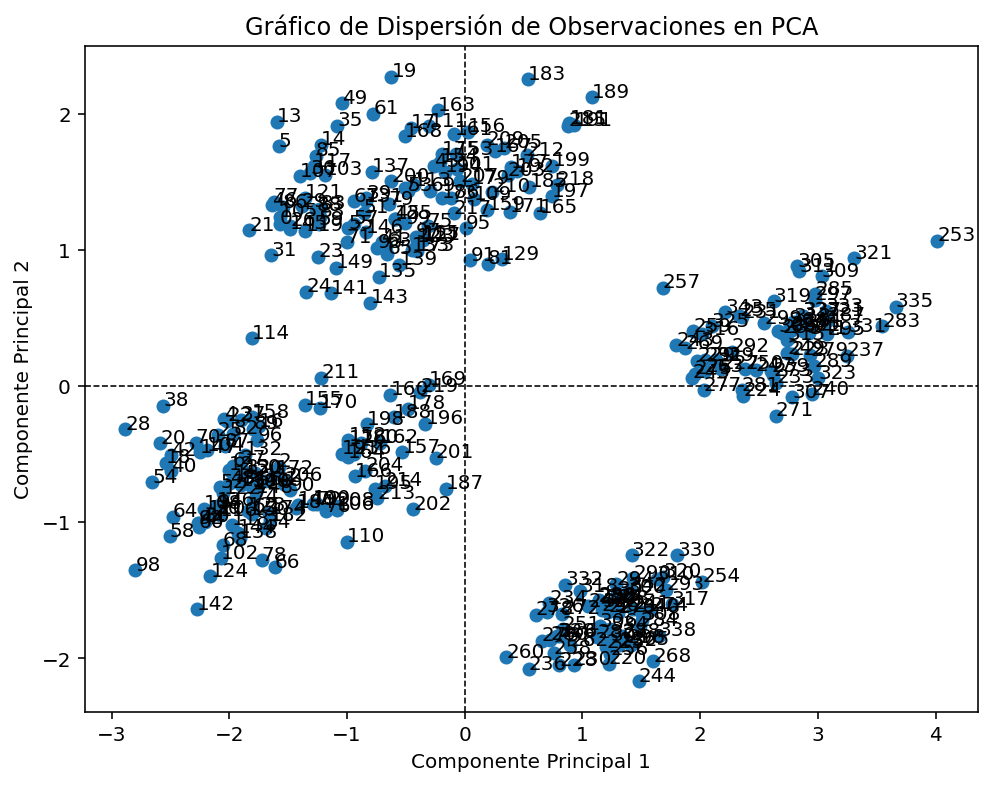
\includegraphics[width=\textwidth]{graficos/dispersionBasico.png}
            \caption{\small{Gráfico de dispersión de las observaciones}}
            \label{fig:dispersionBasico}
        \end{minipage}
        \caption{Conjunto de gráficas}
        \label{fig:multiplesGraficas}
    \end{figure}
\end{center}

\begin{center}
    \begin{figure}[h!]
        \centering
        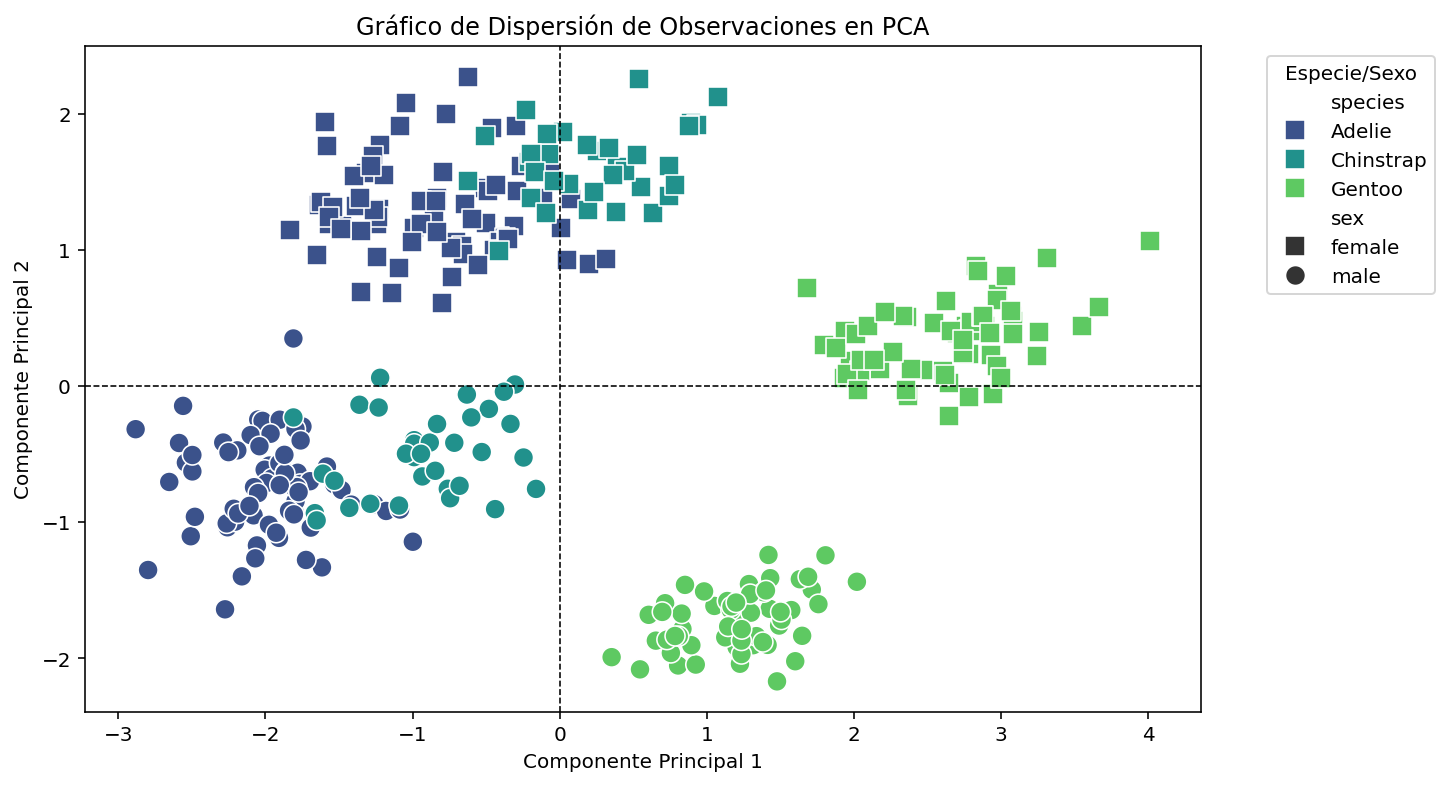
\includegraphics[width=0.7\textwidth]{graficos/dispersionEspecies.png}
        \caption{Gráfico de dispersión por especie}
        \label{fig:dispersionEspecies}
    \end{figure}
\end{center}

Además, en la figura \ref{fig:dispersionEspecies}, podemos ver el mismo gráfico de la figura \ref{fig:dispersionBasico}, pero con cada observación coloreada 
en función de la especie a la que pertenece, y con una forma distinta en función del género del pingüino (y eliminando también el índice de cada pingüino, 
para hacer el gráfico más legible y que se aprecien más las diferencias entre especies). El código de este gráfico, que parte de la función 
\texttt{plot\_pca\_scatter}, puede observarse en \ref{lst:code}.

Inicialmente, observamos cuatro grupos diferenciados, dos de los cuales se corresponden exclusivamente con la especie \textit{Gentoo}. Para esta especie, 
vemos que todos sus individuos presentan un comportamiento similar para la componente 1 (que, como dijimos, está relacionada con el tamaño de los pingüinos). 
Además, curiosamente, los dos subgrupos que se observan se encuentran justo en lados opuestos de la componente 2, que era la que definimos como el marcador 
de género, y podemos observar que todos los Gentoo hembra toman valores de la componente 2 positivos, mientras que los Gentoo macho toman valores negativos. 
Esto nos sugiere nuestras suposiciones iniciales sobre lo que representaba cada componente.

Además, para las especies \textit{Adelie} y \textit{Chinstrap} se observa una situación parecida: ambas toman valores similares para la componente 1, lo que 
nos sugiere que son individuos con características físicas y de peso similares; y están polarizadas, aunque con menos diferencia que los Gentoo, en función 
del género del pingüino. Estas especies son las que destacan menos en la primera componente, o las que destacan más ''negativamente'' (indicando, quizás, 
individuos de menor tamaño que los Gentoo).

\begin{lstlisting}[language=Python, label={lst:code}, caption={Código para la obtención del gráfico de dispersión}]
    penguins_std['species'] = penguins_original['species']
    penguins_std['sex'] = penguins_original['sex'].map({0: 'male', 1: 'female'})

    for i in range(n_components):
        for j in range(i + 1, n_components):
            plt.figure(figsize=(10, 6)) 
            sns.scatterplot(
                x=componentes_principales[:, i], 
                y=componentes_principales[:, j],  
                hue=penguins_std['species'],  # Color por especie
                style=penguins_std['sex'],    # Forma según sexo
                palette='viridis', s=100, 
                markers={'male': 'o', 'female': 's'}  # Marcadores para machos y hembras
            )
            
            plt.axhline(0, color='black', linestyle='--', linewidth=0.8)
            plt.axvline(0, color='black', linestyle='--', linewidth=0.8)
            plt.xlabel(f'Componente Principal {i + 1}')
            plt.ylabel(f'Componente Principal {j + 1}')
            plt.title(f'Gráfico de Dispersión de Observaciones en PCA')
            plt.legend(title='Especie/Sexo', bbox_to_anchor=(1.05, 1), loc='upper left')
            plt.show()
\end{lstlisting}

Para valorar conjuntamente las características físicas de los pingüinos, podemos construir un índice que considere ambas componentes. Una primera aproximación 
podría ser construirlo en base a una combinación ponderada de las dos componentes principales, basándose en el cos2 que tiene cada uno de las componentes 
(que vimos en \ref{PCAinicial}), de forma que tendríamos algo como $Indice = w1*CP1 + w2*CP2$ (donde w1 y w2 son la suma del cos2 para CP1 y CP2). 

Para calcular el índice para, por ejemplo, Adelie, podemos emplear el siguiente código, donde se calcula en primer lugar los valores de las componentes 
principales para esta especie, para a continuación aplicar el índice que hemos calculado. De esta forma, obtenemos un valor de -3.653316 para el índice, lo que 
nos indica que los pingüinos de esta especie tienden a tener valores bajos en ambas componentes, lo que sugiere que son más pequeños en tamaño, con picos menos 
profundos, y menos diferencia entre géneros.

Si repetimos el proceso para Chinstrap, obtenemos un índice de -0.161348, y para Gentoo de 4.574419. Si observamos 
la gráfica \ref{fig:dispersionEspecies}, podemos corroborar esto, ya que vemos que los pingüinos más pequeños son claramente los Adelie, con un tamaño similar 
a los Chinstrap, pero con estos últimos presentando un mayor marcaje de género; mientras que los Gentoo son tanto los más grandes como los que más marcaje de 
género presentan.
\begin{lstlisting}[language=Python]
    w1 = cos2['Componente 1'].sum()  # Peso para CP1
    w2 = cos2['Componente 2'].sum()  # Peso para CP2
    resultados_pca = pd.DataFrame(componentes_principales, columns=['Componente 1', 'Componente 2'])
    resultados_pca['Índice'] = (w1 * resultados_pca['Componente 1']) + (w2 * resultados_pca['Componente 2'])
    
    adelie_data = penguins_std[penguins_std['species'] == 'Adelie']
    adelie_cp = pca.transform(adelie_data.drop(columns=['species', 'sex']))
    adelie_cp_df = pd.DataFrame(adelie_cp, columns=['Componente 1', 'Componente 2'])
    adelie_cp_df['Índice'] = (w1 * adelie_cp_df['Componente 1']) + (w2 * adelie_cp_df['Componente 2'])
    print(f"Índice Adelie: {adelie_cp_df['Índice'].mean()}")
\end{lstlisting}

\section{Clustering} \label{clustering}
\subsection{Agrupamiento jerárquico} \label{jerarquico}
En el clústering jerárquico, haremos las agrupaciones sin conocer de antemano el número de clústers. Esto nos servirá para poder tener una idea del número de 
clústers que se deben elegir, y hacer con ello el análisis no jerárquico. Lo primero que haremos será crear un mapa de calor con los datos, como el que figura 
en la imagen \ref{fig:mapaCalor}. Sin embargo, este mapa no nos ayuda especialmente a encontrar patrones entre las variables, ya que las mismas tienen escalas 
dispares, y vemos que toda la representatividad del gráfico la acapara el peso de los pingüinos. Lo que si nos da una idea, gracias al dendograma que incluye, 
es de que quizás el número de clústers a elegir sería de tres.
\begin{center}
    \begin{figure}[h!]
        \centering
        \begin{minipage}{0.5\textwidth}
            \centering
            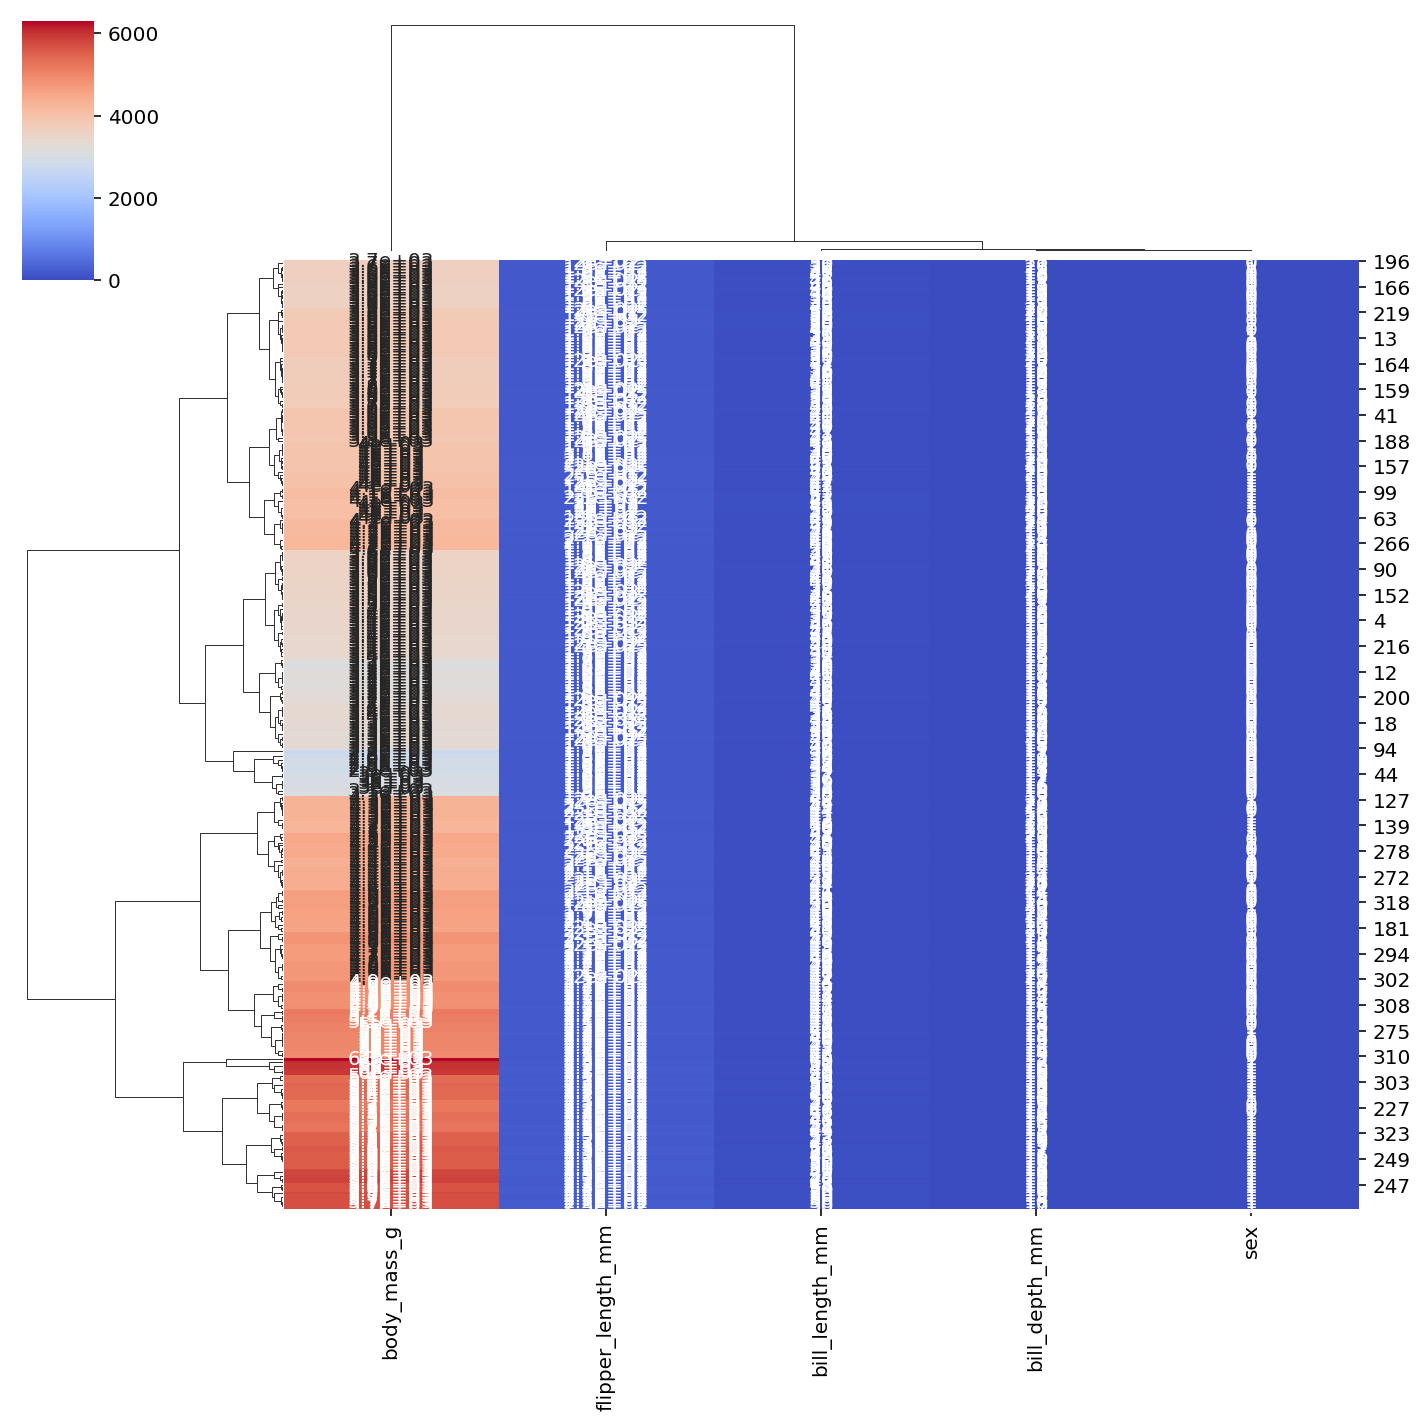
\includegraphics[width=\textwidth]{graficos/mapaCalor.png}
            \caption{\small{Mapa de calor}}
            \label{fig:mapaCalor}
        \end{minipage}
        \hspace{0.005\textwidth} % Espacio entre las imágenes
        \begin{minipage}{0.45\textwidth}
            \centering
            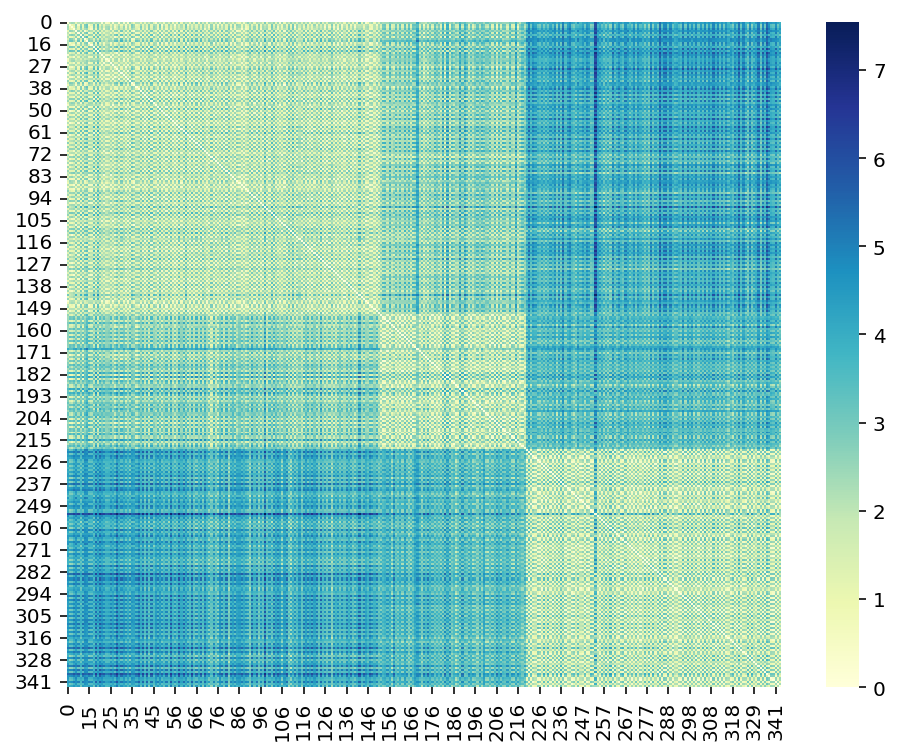
\includegraphics[width=\textwidth]{graficos/matrizDistancias.png}
            \caption{\small{Matriz de distancias}}
            \label{fig:matrizDistancias}
        \end{minipage}
    \end{figure}
\end{center}

En la figura \ref{fig:matrizDistancias} se ve también la matriz de distancias, obtenida a partir de las distancias euclidianas, representada de forma gráfica 
y coloreada. En ella se podrían observar, a priori, dos o tres grupos de variables con distancias similares. Si reorganizamos la matriz, para obtener una 
mejor visualización de cuáles son los grupos y poder analizar mejor los patrones, obtenemos la figura \ref{fig:matrizEnlace}. Aquí, se observa que quizás 
el número de clústers podría ser entre 4 y 5, ya que son los distintos grupos que se observan en dicha matriz.
\begin{center}
    \begin{figure}[h!]
        \centering
        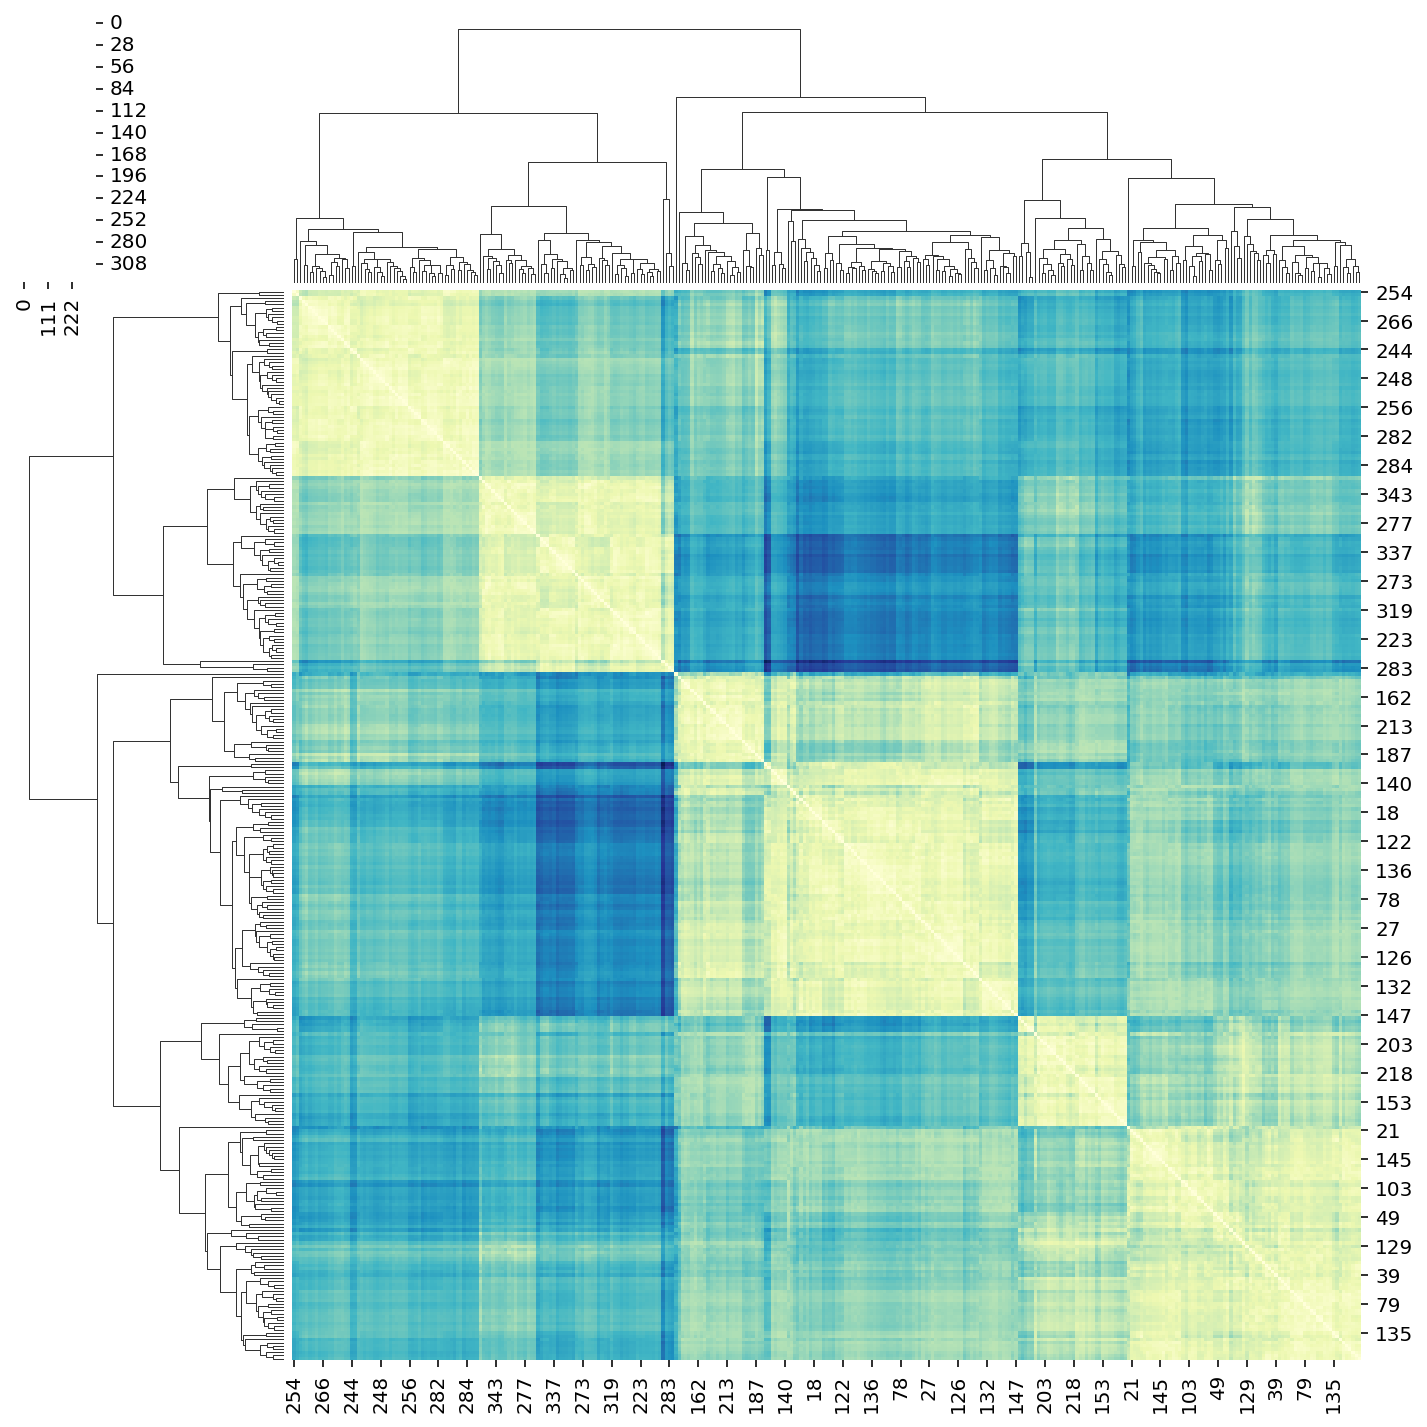
\includegraphics[width=0.5\textwidth]{graficos/matrizEnlace.png}
        \caption{Matriz de distancias ordenada}
        \label{fig:matrizEnlace}
    \end{figure}
\end{center}

Para concluir con el agrupamiento jerárquico, obtenemos el dendrograma, un diagrama con estructura de árbol que nos muestra los resultados de la agrupación. 
Para ello, el dendrograma parte de tantos grupos como observaciones haya, y los va uniendo hasta obtener un único grupo. Así, la altura a la que se unen los 
grupos representa la distancia entre los mismos, por lo que cuanto menor sea la distancia más similares son los grupos. Esto será lo que nos ayude a decidir 
el número de grupos óptimo para emplear en el análisis no jerárquico. En nuestro caso, obtenemos el dendrograma de la figura \ref{fig:dendrograma}, al cual le 
hemos establecido un límite para la altura de 15, ya que parece ser la óptima. Así, el dendrograma nos sugeriría crear 4 grupos. Podría hilarse incluso más 
fino, y establecer la altura máxima a 10, lo cual nos sugeriría el uso de 6 clústers. Sin embargo, se opta por elegir 4, ya que parece que explica más los 
datos observados en los gráficos \ref{fig:dispersionBasico} y \ref{fig:dispersionEspecies}, con 4 grupos diferenciados (aunque, con 6 grupos, podría sugerirnos 
tener un grupo por cada especie y género, lo cual podría resultar también interesante).
\begin{center}
    \begin{figure}[h!]
        \centering
        \begin{minipage}{0.45\textwidth}
            \centering
            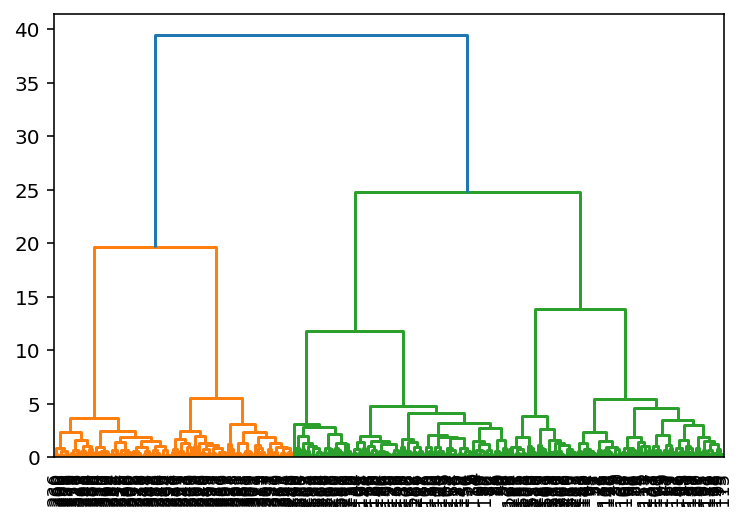
\includegraphics[width=\textwidth]{graficos/dendograma.png}
            \caption{Dendrograma}
            \label{fig:dendrograma}
        \end{minipage}
        \hspace{0.005\textwidth} % Espacio entre las imágenes
        \begin{minipage}{0.5\textwidth}
            \centering
            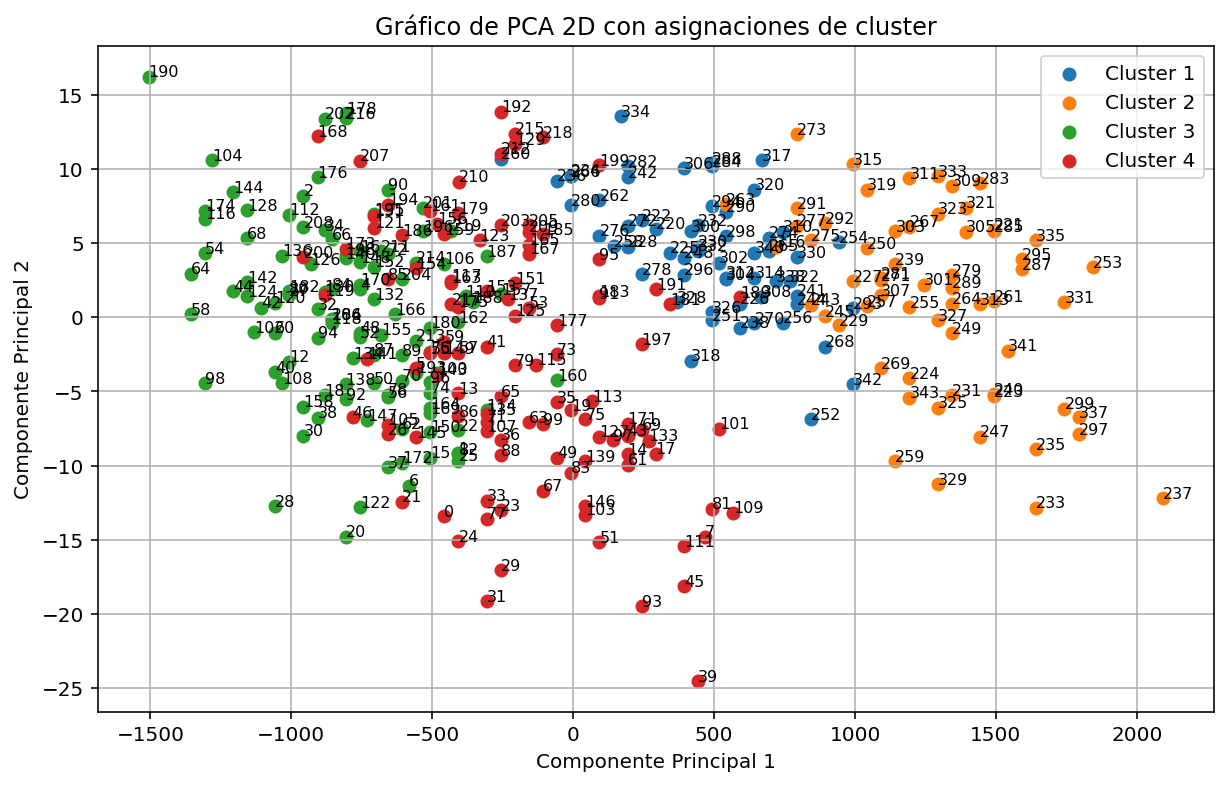
\includegraphics[width=\textwidth]{graficos/PCAClusters.png}
            \caption{PCA con clústers}
            \label{fig:PCACluster}
        \end{minipage}
    \end{figure}
\end{center}

Una vez definido 4 como el número de grupos, se realiza de nuevo el PCA con dos componentes, para representar los individuos y el clúster al que pertenecen,
obteniendo el grafico \ref{fig:PCACluster}, donde se observan claramente dos grupos diferenciados, dentro de los cuales hay dos respectivos subgrupos: el 1 y el 2,
claramente diferenciados; y el 3 y 4, que si bien se diferencian de los otros dos grupos, están más entremezclados entre si.

\subsection{Agrupamiento K-means} \label{kmeans}
A continuación se procederá con el agrupamiento no jerárquico, que en este caso se hace con el algoritmo de K-means. Este algoritmo parte de un número 
predefinido de clústers (4, en nuestro caso), y selecciona 4 puntos como centroides iniciales. A partir de ahí, va asignando cada punto al clúster cuyo centroide 
tenga más cerca, recalculando el nuevo centroide con cada nueva adición que realiza, hasta que se cumpla un criterio de convergencia, que suele ser un 
número determinado de iteraciones o que los centroides no cambien significativamente.
\begin{center}
    \begin{figure}[h!]
        \centering
        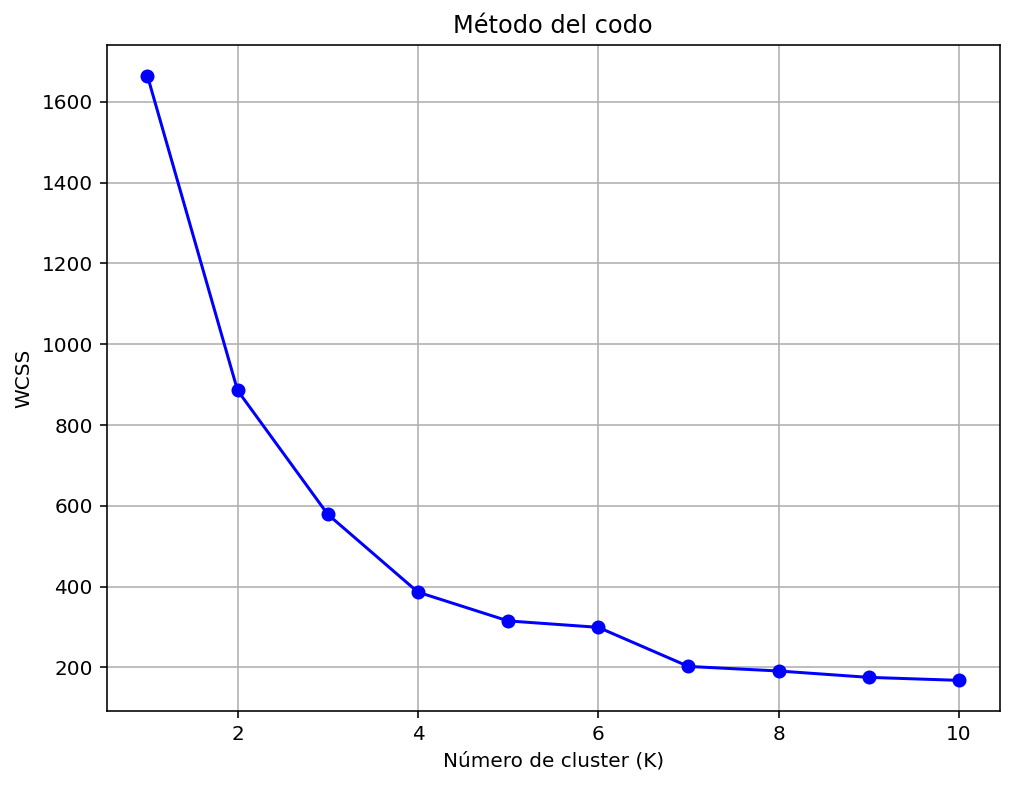
\includegraphics[width=0.5\textwidth]{graficos/metodoCodo.png}
        \caption{Gráfico del método del codo}
        \label{fig:metodoCodo}
    \end{figure}
\end{center}
Pero primero, emplearemos el método del codo, para ver si quizás nuestros 4 grupos que nos habíamos planteado son el número adecuado, o deberíamos ampliarlo 
o reducirlo. Este método calcula el WCSS o la suma de cuadrados dentro del grupo (cuánto de lejos están los puntos dentro de un grupo a su respectivo centroide), 
para diferentes valores de k, y los grafica, dando como resultado una curva que tiende a disminuir cuanto mayor es k. Se busca el punto de codo, donde el WCSS 
comienza a disminuir más lentamente, lo que nos dice que es el número ideal de grupos. En nuestro caso, observamos claramente el codo en $k=4$, por lo que 
ese número de clústers es el óptimo. Aplicamos entonces el método K-means con estos 4 clústers, y realizamos la representación de los individuos y el clúster 
al que pertenecen (figura \ref{fig:KMEANS4}). Se observa un caso similar al comentado en \ref{jerarquico}, con dos grupos diferenciados entre si, y dos subgrupos 
a su vez, también diferenciados entre sí.
\begin{center}
    \begin{figure}[h!]
        \centering
        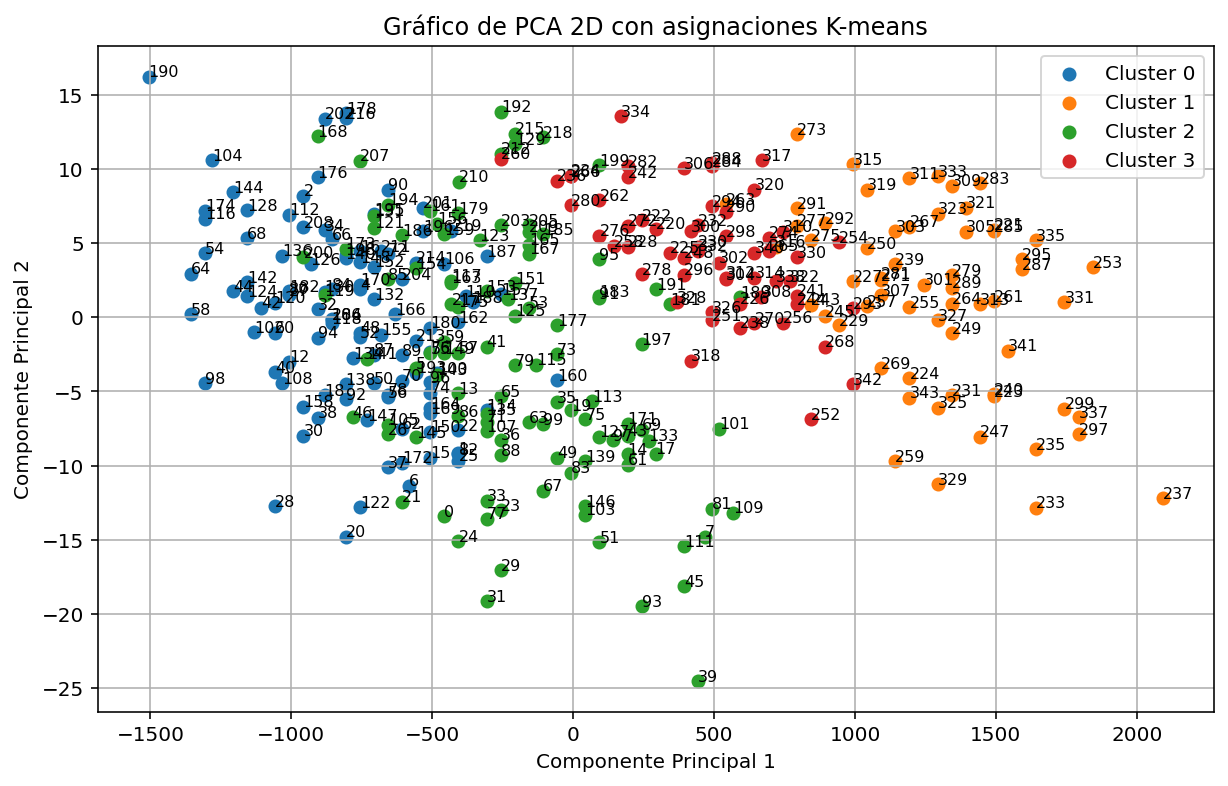
\includegraphics[width=0.6\textwidth]{graficos/PCAKmeans4.png}
        \caption{Agrupamiento K-means con 4 clústers}
        \label{fig:KMEANS4}
    \end{figure}
\end{center}

Sin embargo, como vimos en el \hyperref[fig:metodoCodo]{gráfico del codo}, aunque el descenso brusco se produce en 4 clústers, vemos una especie de ''escalón'' 
en $k=6$. Podría resultar interesante realizar también el agrupamiento K-means en 6 clústers, para representarlo gráficamente, y ver como se distribuyen los 
pingüinos en los grupos (aunque posteriormente realizaremos la \hyperref[validacion]{validación del agrupamiento} aplicando la puntuación de silueta). Si vemos 
ahora el gráfico \ref{fig:KMEANS6}, vemos que los dos primeros grupos se mantienen intactos, y los otros dos se han subdividido. Sin embargo, no se aprecian 
marcadas diferencias entre los individuos; es más, no están definidos claramente. Por tanto, podemos concluir que el criterio de emplear 4 clústers es el correcto.
\begin{center}
    \begin{figure}[h!]
        \centering
        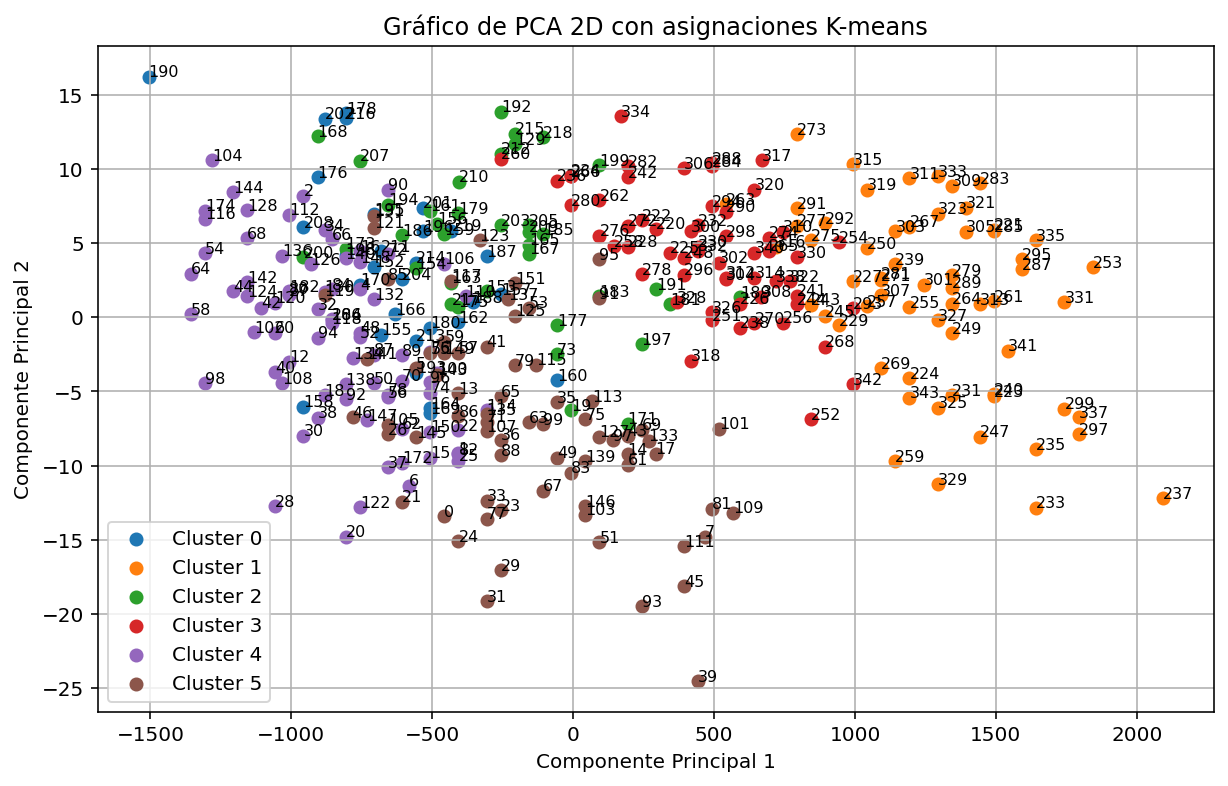
\includegraphics[width=0.6\textwidth]{graficos/PCAKmeans6.png}
        \caption{Agrupamiento K-means con 6 clústers}
        \label{fig:KMEANS6}
    \end{figure}
\end{center}

\subsection{Validación del agrupamiento} \label{validacion}
Para validar la calidad del agrupamiento, además del método que ya vimos del codo, emplearemos la puntuación de silueta. Este método se basa en calcular, por 
una parte, la distancia media de cada observación a los demás puntos del mismo grupo (denotado como $a$), y a todos los puntos del clúster mças cercano al que 
no pertenezca la observación (denotado como $b$), y calculando la puntuación de silueta para esa observación como el cociente de $b-a$ y el máximo entre ambas. 
Repitiendo esto para todas las observaciones, obtenemos la puntuación general de silueta, que varía entre -1 y 1, donde una puntuación cercana a 1 indica que 
la observación coincide bien con su grupo y se diferencia bien de los demás. Por tanto, se debe buscar aquel número de agrupaciones en el que la puntuación 
de silueta sea mayor. Esto lo hemos graficado en la figura \ref{fig:silueta}, donde vemos en primer lugar un máximo local en $k=4$, mientras que el máximo 
absoluto es en $k=6$. Esto nos indica que el número óptimo de clústers sería o bien 4 o 6. Sin embargo, teniendo en cuenta también lo visto en el método del 
codo, y combinando ambas observaciones, podemos concluír que el número óptimo de clústers es 4.
\begin{center}
    \begin{figure}[h!]
        \centering
        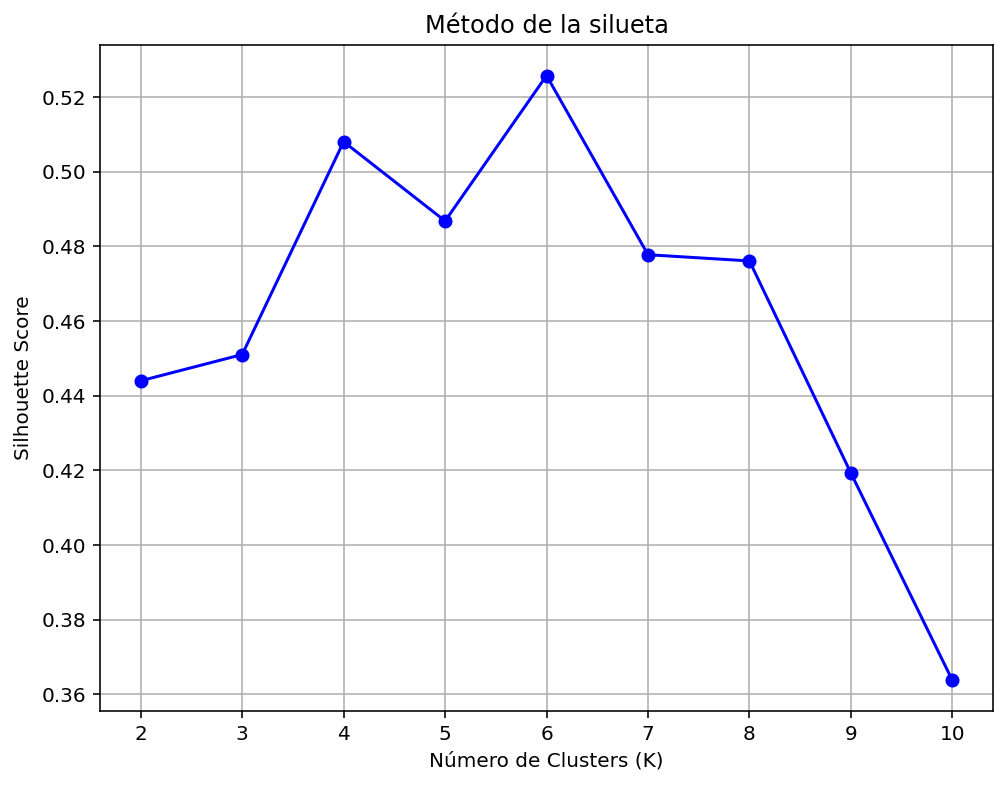
\includegraphics[width=0.5\textwidth]{graficos/metodoSilueta.png}
        \caption{Gráfico de la puntuación de silueta}
        \label{fig:silueta}
    \end{figure}
\end{center}

Por último, en la figura \ref{fig:siluetaClusters} observamos los valores de silueta dentro de cada cluster. Lo primero que se observa es que no hay ningún 
valor negativo, por lo que las puntuaciones de silueta son buenas, sugiriendo que no hay ninguna observación que habría pertenecido a otro grupo. El grupo más 
dispar es el 0 (coloreado en morado), ya que es en el que se ve más variación entre las puntuaciones de silueta. Los grupos 3 y 1 serían los más homogéneos, 
los que menos diferencias tienen, pero también son los que menos observaciones tienen. Por último, tendríamos el grupo 1, también con gran 
variación entre las puntuaciones, pero ligeramente menor que la del grupo 0, y con una puntuación media más baja.
\begin{center}
    \begin{figure}[h!]
        \centering
        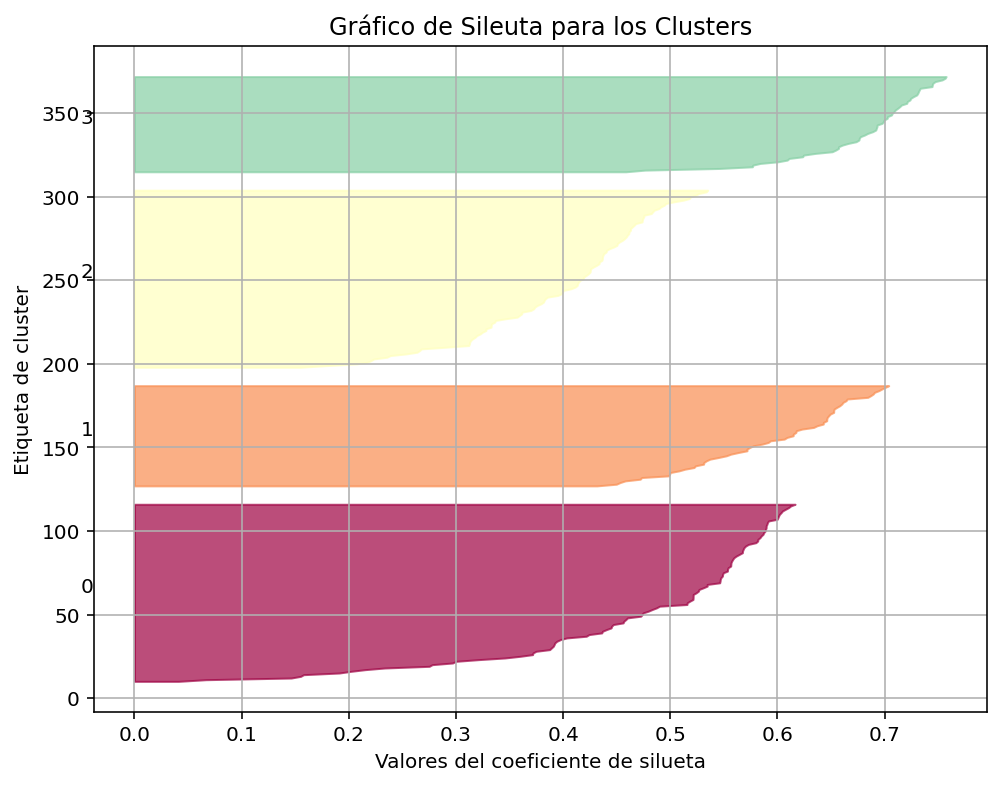
\includegraphics[width=0.6\textwidth]{graficos/siluetaPuntuaciones.png}
        \caption{Puntuación de silueta para cada clúster}
        \label{fig:siluetaClusters}
    \end{figure}
\end{center}

\subsection{Comparación entre agrupamiento jerárquico y K-means} \label{comparacion}
\begin{center}
    \begin{figure}[h!]
        \centering
        \begin{minipage}{0.49\textwidth}
            \centering
            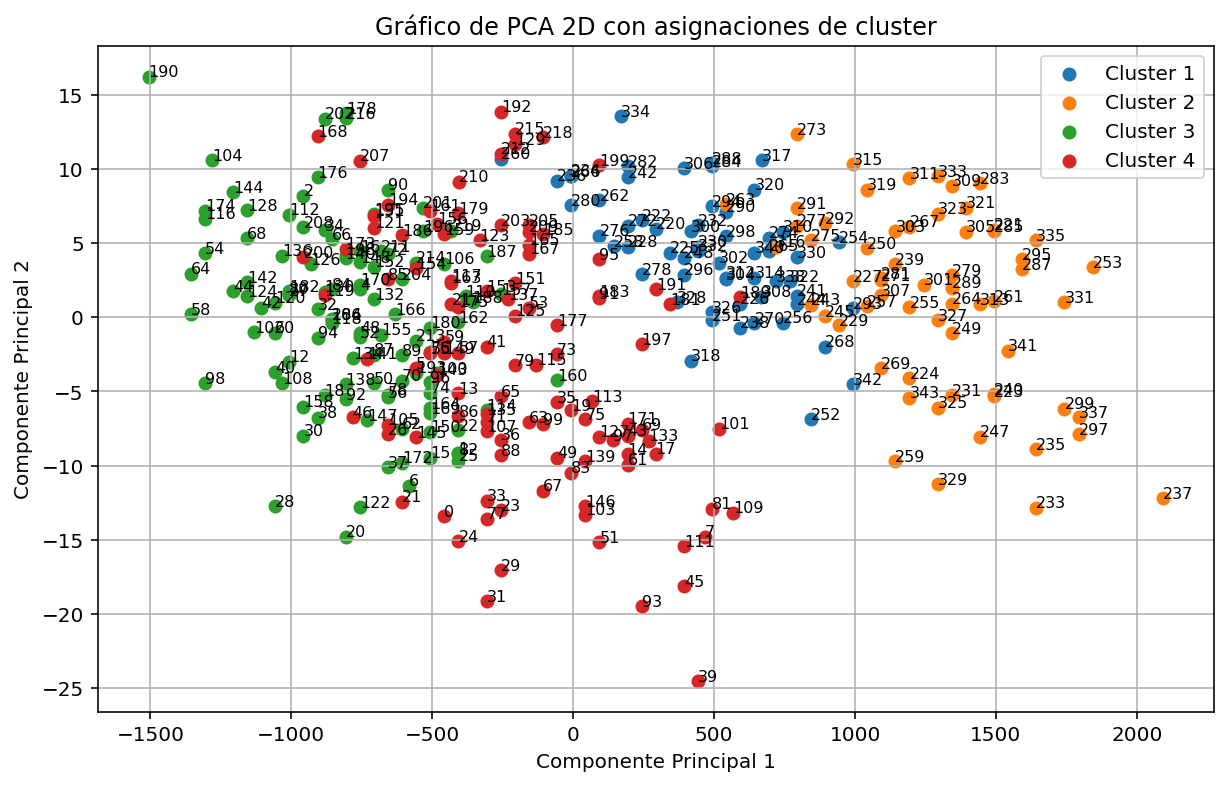
\includegraphics[width=\textwidth]{graficos/PCAClusters.png}
            Figura \ref{fig:PCACluster}
        \end{minipage}
        \hspace{0.005\textwidth} % Espacio entre las imágenes
        \begin{minipage}{0.49\textwidth}
            \centering
            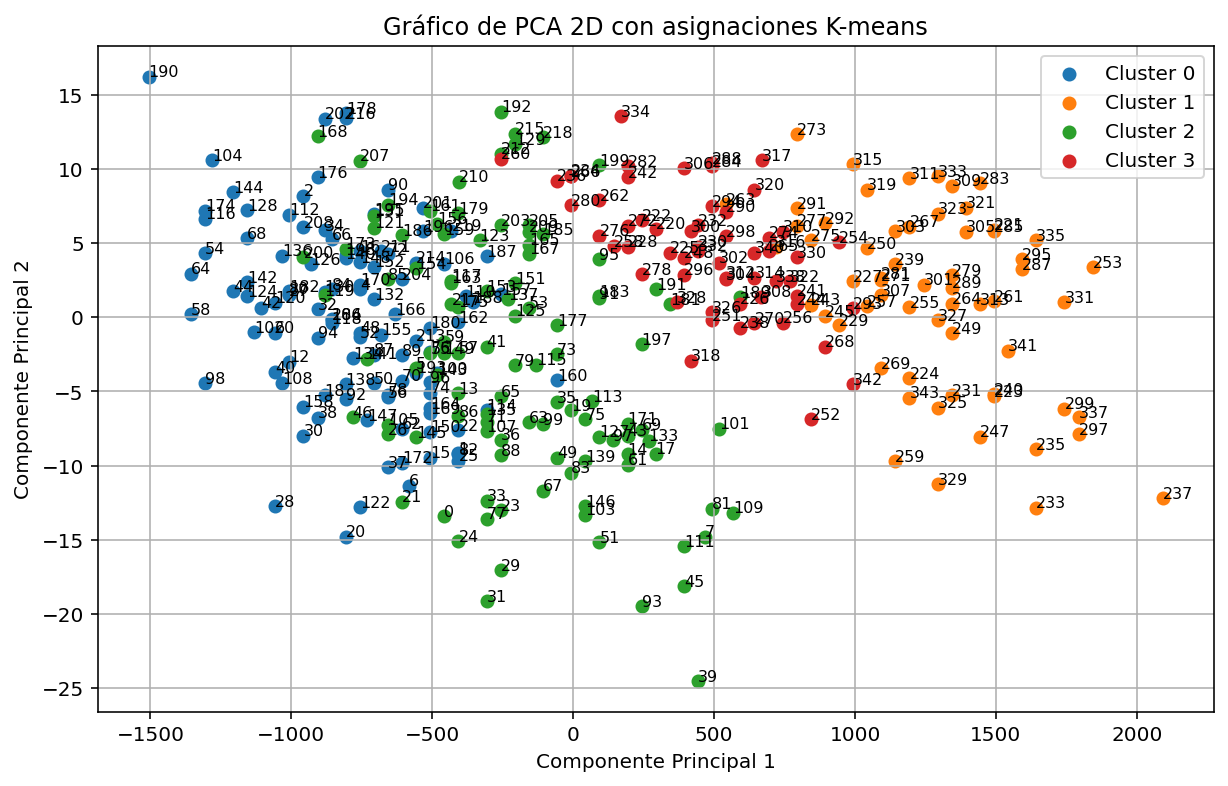
\includegraphics[width=\textwidth]{graficos/PCAKmeans4.png}
            Figura \ref{fig:KMEANS4}
        \end{minipage}
    \end{figure}
\end{center}
Para la comparación entre agrupamientos rescatamos en este punto las figuras \ref{fig:PCACluster}, que representa las asignaciones del agrupamiento jerárquico;
y la figura \ref{fig:KMEANS4}, con las asignaciones del método de K-means, lo que facilitará el análisis. En este caso, el análisis es muy sencillo, ya que 
se observa una gran concordancia, puesto que exactamente todos los puntos pertenecen a los mismos clústers, tanto en el jerárquico como en el K-means 
(teniendo en cuenta que en uno los grupos se numeran del 1 al 4, y en otro del 0 al 3). Esto significa que la estructura de los datos es lo suficientemente clara 
y está separada lo suficiente como para que ambos algoritmos detecten los mismos patrones en las agrupaciones.

\section{Interpretación de los resultados} \label{resultados}
En primer lugar, representamos los centroides de cada uno de los clústers sobre las observaciones originales, en la figura \ref{fig:centroides}.
\begin{center}
    \begin{figure}[h!]
        \centering
        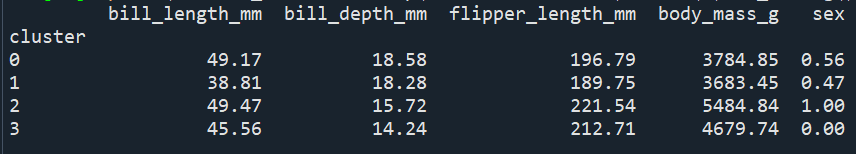
\includegraphics[width=0.8\textwidth]{graficos/centroides.png}
        \caption{Centroides de los clústers}
        \label{fig:centroides}
    \end{figure}
\end{center}
En las figuras \ref{fig:aggrSencilla} tenemos el recuento de los pingüinos que hay en cada clúster por especie y por isla, mientras que en la figura 
\ref{fig:aggrSex} lo tenemos además dividido por sexos.
\begin{center}
    \begin{figure}[h!]
        \centering
        \begin{minipage}{0.4\textwidth}
            \centering
            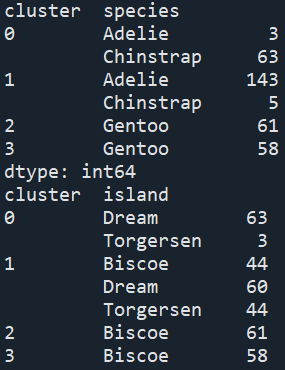
\includegraphics[width=\textwidth]{graficos/agrupacionSencilla.png}
            \caption{Recuento de los clústers}
            \label{fig:aggrSencilla}
        \end{minipage}
        \hspace{0.005\textwidth} % Espacio entre las imágenes
        \begin{minipage}{0.4\textwidth}
            \centering
            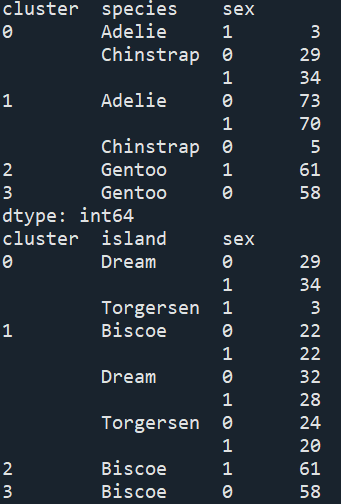
\includegraphics[width=\textwidth]{graficos/agrupacionConSex.png}
            \caption{Recuento de los clústers con agrupación por sexo}
            \label{fig:aggrSex}
        \end{minipage}
    \end{figure}
\end{center}

A partir de los centroides, podemos concluir que el agrupamiento que se ha realizado ha identificado correctamente grupos con diferencias morfológicas 
significativas, tanto a nivel de especie, como de isla, como de sexo.

A nivel de especies, los pingüinos Gentoo están claramente diferenciados en los clústers 2 y 3, lo cual sugiere que son los que más se diferencian respecto a 
las otras especies. Además, cada uno de estos clústers se corresponde con un sexo de pingüinos distintos: en el clúster 2, pingüinos Gentoo macho, y en el 
clúster 3, pingüinos Gentoo hembra. Esto nos indica que el dimorfismo sexual en los pingüinos de esta especie es claramente marcado, y que las hembras  de esta 
especie tienden a pesar menos y tener la aleta más corta. Por otra parte, las especies de Adelie y Chinstrap se encuentran mezcladas en los clústers 0 y 1, pero 
con una notable predominancia en el primero de los Chinstrap (63 ejemplares, por 3 de los Adelie), mientras el segundo está dominado por los Adelie (143, por 
5 de los Chinstrap). Esto indica que estas especies son morfológicamente similares, o que comparten bastantes características (como un peso muy bajo en ambos 
casos), pero con diferencias en cuanto a la longitud del pico (que es más largo en el primer grupo) que el agrupamiento consigue diferenciar correctamente.

A nivel de islas, tenemos la misma situación que antes con los Gentoo. La isla Biscoe predomina en los clústers 2 y 3, aunque también hay numerosos ejemplares 
en el clúster 1. Esto, combinado con lo que vimos anteriormente, nos sugiere que Gentoo podría ser la especie predominante en esta isla. Por otra parte, la isla 
Dream, asociada mayoritariamente en el clúster 0, donde Chinstrap era la especie dominante. Por último, la isla Torgersen, mayoritaria en el clúster 1, que 
nos indica que está habitada principalmente por los Adelie.

Respecto a las características morfológicas de los clústers, el clúster 0 se caracteriza por tener pingüinos con un pico largo y profundo, con aletas de longitud 
intermedia y un peso también intermedio, y con una proporción mayor de machos (ya que el sexo es 0.56). En el clúster 1 tenemos los pingüinos con el pico más 
corto, pero más profundo a su vez, que tienen la aleta más corta de todas y el menor peso, siendo mayoritarios en este clúster las hembras (0.47). El clúster 
2 es íntegramente de pingüinos machos, como vimos anteriormente, de la especie de Gentoo, mientras que el 3 es íntegramente de hembras de esta especie. En esta 
especie, los machos son mucho más pesados que las hembras (1kg), con aletas unos 10mm mayores, pero morfologías de pico similares (apenas 1 milímetro más 
profundos y 4 milímetros más largos).

En resumen, el algoritmo nos ha permitido identificar patrones claros en las especies de pingüinos, quedando claramente establecida una diferencia entre los 
Gentoo y el resto de especies. La superposición que se observa entre Adelie y Chinstrap nos indica que son especies bastante similares morfológicamente, ya 
que el algoritmo no es capaz de separarlas por completo. La distribución por islas también es bastante marcada, con los Gentoo dominantes en Biscoe, y los Adelie 
y Chinstrap distribuidos en las otras dos islas. Este análisis nos puede servir como base para futuras investigaciones que incluyan, por ejemplo, nuevas 
variables, o una mayor cantidad de observaciones, que permita al algoritmo establecer bien las diferencias entre las especies Adelie y Chinstrap para poder 
capturarlas en diferentes clústers.

\end{sloppypar}
\end{document}
